\documentclass[12pt, a4paper]{report}

%%%%%%%%%%%%%%%%%%%%%%%%%%%%%%%%%%%%%% PACKAGES %%%%%%%%%%%%%%%%%%%%%%%%%%%%%%%%
\usepackage[swedish]{babel}
\usepackage[utf8]{inputenc}
\usepackage[hidelinks]{hyperref}
\usepackage{
  amsmath,
  amssymb,
  caption,
  color,
  csquotes,
  float,
  graphicx,
  listings,
  parskip,
  pdflscape,
  pgfgantt,
  scrextend,
  siunitx,
  tikz,
  titlesec,
}
\usepackage[
    backend=biber,
    style=ieee,
	citestyle=numeric-comp,
    sorting=none
]{biblatex}
\addbibresource{refs.bib}
\usetikzlibrary{positioning}

%%%%%%%%%%%%%%%%%%%%%%%%%%%%% LISTINGS SETTINGS %%%%%%%%%%%%%%%%%%%%%%%%%%%%%%%%

\definecolor{mygreen}{rgb}{0,0.4,0.1}
\definecolor{mygray}{rgb}{0.5,0.5,0.5}
\definecolor{mymauve}{rgb}{0.58,0,0.82}

\lstset{
  backgroundcolor=\color{white},   % choose the background color; you must add \usepackage{color} or \usepackage{xcolor}; should come as last argument
  basicstyle=\ttfamily,            % the size of the fonts that are used for the code
  breakatwhitespace=false,         % sets if automatic breaks should only happen at whitespace
  breaklines=true,                 % sets automatic line breaking
  captionpos=b,                    % sets the caption-position to bottom
  commentstyle=\color{mygreen},    % comment style
  deletekeywords={...},            % if you want to delete keywords from the given language
  escapeinside={\%*}{*)},          % if you want to add LaTeX within your code
  extendedchars=true,              % lets you use non-ASCII characters; for 8-bits encodings only, does not work with UTF-8
  firstnumber=1,                   % start line enumeration with line 1000
  frame=single,                    % adds a frame around the code
  keepspaces=true,                 % keeps spaces in text, useful for keeping indentation of code (possibly needs columns=flexible)
  keywordstyle=\color{blue},       % keyword style
  language=c,                      % the language of the code
  morekeywords={*,...},            % if you want to add more keywords to the set
  numbers=none,                    % where to put the line-numbers; possible values are (none, left, right)
  numbersep=5pt,                   % how far the line-numbers are from the code
  numberstyle=\tiny\color{mygray}, % the style that is used for the line-numbers
  rulecolor=\color{black},         % if not set, the frame-color may be changed on line-breaks within not-black text (e.g. comments (green here))
  showspaces=false,                % show spaces everywhere adding particular underscores; it overrides 'showstringspaces'
  showstringspaces=false,          % underline spaces within strings only
  showtabs=false,                  % show tabs within strings adding particular underscores
  stepnumber=2,                    % the step between two line-numbers. If it's 1, each line will be numbered
  stringstyle=\color{mymauve},     % string literal style
  tabsize=2,                       % sets default tabsize to 2 spaces
  title=\lstname                   % show the filename of files included with \lstinputlisting; also try caption instead of title
}

% FIX LISTINGS ENCODING PROBLEM
\lstset{literate=
  {á}{{\'a}}1 {é}{{\'e}}1 {í}{{\'i}}1 {ó}{{\'o}}1 {ú}{{\'u}}1
  {Á}{{\'A}}1 {É}{{\'E}}1 {Í}{{\'I}}1 {Ó}{{\'O}}1 {Ú}{{\'U}}1
  {à}{{\`a}}1 {è}{{\`e}}1 {ì}{{\`i}}1 {ò}{{\`o}}1 {ù}{{\`u}}1
  {À}{{\`A}}1 {È}{{\`E}}1 {Ì}{{\`I}}1 {Ò}{{\`O}}1 {Ù}{{\`U}}1
  {ä}{{\"a}}1 {ë}{{\"e}}1 {ï}{{\"i}}1 {ö}{{\"o}}1 {ü}{{\"u}}1
  {Ä}{{\"A}}1 {Ë}{{\"E}}1 {Ï}{{\"I}}1 {Ö}{{\"O}}1 {Ü}{{\"U}}1
  {â}{{\^a}}1 {ê}{{\^e}}1 {î}{{\^i}}1 {ô}{{\^o}}1 {û}{{\^u}}1
  {Â}{{\^A}}1 {Ê}{{\^E}}1 {Î}{{\^I}}1 {Ô}{{\^O}}1 {Û}{{\^U}}1
  {ã}{{\~a}}1 {ẽ}{{\~e}}1 {ĩ}{{\~i}}1 {õ}{{\~o}}1 {ũ}{{\~u}}1
  {Ã}{{\~A}}1 {Ẽ}{{\~E}}1 {Ĩ}{{\~I}}1 {Õ}{{\~O}}1 {Ũ}{{\~U}}1
  {œ}{{\oe}}1 {Œ}{{\OE}}1 {æ}{{\ae}}1 {Æ}{{\AE}}1 {ß}{{\ss}}1
  {ű}{{\H{u}}}1 {Ű}{{\H{U}}}1 {ő}{{\H{o}}}1 {Ő}{{\H{O}}}1
  {ç}{{\c c}}1 {Ç}{{\c C}}1 {ø}{{\o}}1 {å}{{\r a}}1 {Å}{{\r A}}1
  {€}{{\euro}}1 {£}{{\pounds}}1 {«}{{\guillemotleft}}1
  {»}{{\guillemotright}}1 {ñ}{{\~n}}1 {Ñ}{{\~N}}1 {¿}{{?`}}1 {¡}{{!`}}1
}

%%%%%%%%%%%%%%%%%%%%%%%%%%%%%%%  NICE PALETTE  %%%%%%%%%%%%%%%%%%%%%%%%%%%%%%%%%

% https://images.squarespace-cdn.com/content/v1/638773c92dfb4812d5f5ff28/1669823793535-UWL204TLLHME6SFDP2QZ/image-asset.png
\definecolor{navy}{RGB}{16,37,38}
\definecolor{ginger}{RGB}{205,126,89}
\definecolor{seafoam}{RGB}{69,115,115}
\definecolor{sunflower}{RGB}{221,178,71}
\definecolor{jean}{RGB}{90,104,104}


%%%%%%%%%%%%%%%%%%%%%%%%%%%%%%%%%% HACKS %%%%%%%%%%%%%%%%%%%%%%%%%%%%%%%%%%%%%%%

% Change \chapter format
\titleformat{\chapter} % command
    [display] % shape
  {\normalfont\huge\bfseries} % format
  {} % label
  {0pt} % sep
  {\Huge\thechapter\quad} % before-code
  [] % after code
\titleformat{name=\chapter,numberless} % command
    [display] % shape
  {\normalfont\huge\bfseries} % format
  {} % label
  {0pt} % sep
  {\Huge} % bfore-code
  [] % after-code
\titlespacing*{\chapter}
    {0pt}  % left
    {-1cm} % before
    {0pt}  % after

%%%%%%%%%%%%%%%%%%%%%%%%%%%%%%%%%  TITLE PAGE  %%%%%%%%%%%%%%%%%%%%%%%%%%%%%%%%%

%\title{Projektrapport - Binäranalys med en hybrid av automatiska och manuella metoder}
%\author{
%    Loke Gustafsson \and
%    Samuel Kyletoft \and
%    Enayatullah Norozi \and
%    Albin Otterhäll \and
%    Clara Salberg \and
%    Linus Wallman
%}
%\date{2023-02-20}

%%%%%%%%%%%%%%%%%%%%%%%%%%%%%%%%%% COMMANDS %%%%%%%%%%%%%%%%%%%%%%%%%%%%%%%%%%%%
\newcommand{\stoe}{S$^2$E}

%%%%%%%%%%%%%%%%%%%%%%%%%%%%% DOCUMENT STRUCTURE %%%%%%%%%%%%%%%%%%%%%%%%%%%%%%%

\begin{document}
\pagenumbering{gobble} % turn off page numbers

%%% Cover image %%%
\vtop{
    \null\vspace{-25mm}
    \centerline{
\includegraphics[width=1\textwidth]{figures/chalmers_gu_logo.jpg}}
    \vspace{0.5mm}
    \rule{\textwidth}{1pt}
}

%%% Cover text %%%
\mbox{}
\vfill
\textbf{{\Huge Binäranalys med en hybrid av automatiska och manuella metoder}} \\[0.5cm]
Bachelor of Science Thesis in Computer Science and Engineering \setlength{\parskip}{1cm}

\noindent
{\Large Loke Gustafsson, Samuel Kyletoft, Enayatullah Norozi, Albin Otterhäll,
Clara Salberg, Linus Wallman} \setlength{\parskip}{1.5cm}

%%% Cover footer %%%

\rule{\textwidth}{1pt}
\textsc{Chalmers University of Technology} \\
\textsc{University of Gothenburg} \\
{\small Department of Computer Science and Engineering} \\
{\small Gothenburg, Sweden \the\year \\


\newpage
% TITLE PAGE
\newpage
\thispagestyle{empty}
\begin{center}

	\textbf{\Large \ambaTitle} \\[1cm]

    {\linespread{1.2}\large
        \StrSubstitute{\ambaAuthors}{,}{\\}
        \\
    }
	
	\vfill 	

	\ambaDepartment \\
	\textsc{Chalmers University of Technology} \\
	\textsc{University of Gothenburg} \\
	\ambaCityCountryYear
\end{center}


\newpage
%\thispagestyle{plain}
%\vspace*{4.5cm}
{The authors grant to Chalmers University of Technology and University of Gothenburg the
non-exclusive right to publish the work electronically and in a non-commercial purpose make it
accessible on the Internet. The authors warrant that they are the authors to the work, and
warrant that the work does not contain text, pictures or other material that violates
copyright law.
The authors shall, when transferring the rights of the work to a third party (for example a
publisher or a company), acknowledge the third party about this agreement. If the authors have
signed a copyright agreement with a third party regarding the work, the authors warrant
hereby that they have obtained any necessary permission from this third party to let Chalmers
University of Technology and University of Gothenburg store the work electronically and make
it accessible on the Internet.}

Supervisor: Iulia Bastys \\
Examiner: Joachim von Hacht \setlength{\parskip}{1cm}

Chalmers University of Technology\\
University of Gothenburg\\
\ambaDepartment \\
SE-412 96 Gothenburg\\
Telephone +46 31 772 1000 \setlength{\parskip}{0.5cm}

\vfill
\ambaCityCountryYear


\newpage
\pagenumbering{roman} % turn on roman page numbers
\setcounter{page}{3}

\tableofcontents
\newpage

\addcontentsline{toc}{section}{Begreppslista}
\chapter*{Begreppslista}
\begin{labeling}{begreppslista}

    \item [\textbf{Assembler}] Assembler (jfr.\ eng.\ \emph{assembly}) är ett
    lågnivåspråk som direkt kan översättas till maskinkod.

    \item[\textbf{Basic block}] \emph{Basic block} (jfr.\ sv.\ grundblock) är en
    sekvens av instruktioner som saknar hopp eller förgreningar bortsett från
    början och slutet av blocket. Är oftast expanderade till att bli så långa
    som möjligt

    \item [\textbf{Black-box analys}] Black-box analys (jfr.\ sv.\
    svartlådeanalys) är en analys av ett objekt som endast betraktar dess
    yttre utseende och beteende, till skillnad från white-box-analys som även
    betraktar vad som händer inuti.

    \item [\textbf{Binär}] En binär (jfr.\ eng.\ \emph{binary}) är en fil som
    innehåller ett programs maskinkod och data.

    \item [\textbf{Återanropsfunktion}] Återanropsfunktion (jfr.\ eng.\
    \emph{callback function}) är funktioner som läggs i en \emph{hook} (jfr.\ sv.\ krok) för
    att exekveras vid ett visst tillstånd.

    \item [\textbf{CTF}] CTF (\emph{Capture the Flag}, jfr.\ sv.\ fånga
    flaggan) är i datorsäkerhetssammanhang är en utmaning eller övning i att
    hitta gömda ''flaggor'' i program med avsiktliga säkerhetshål.

    \item [\textbf{Dynamisk analys}] Dynamisk analys (jfr.\ eng.\ \emph{dynamic
        analysis}) är när en binär analyserar genom att exevera binären i en
    kontrollerad miljö för att i detalj registrera vad binären gör.

    \item [\textbf{ELF}] ELF (\emph{Executable and Linkable Format}, jfr.\ sv.\
    exekverbart och länkbart format). Filformatet för exekverbara filer
    på Linux och liknande system. Innehåller maskinkod och länkar till andra
    ELF-filer.

    \item [\textbf{Exekveringsmotor}] En exekveringsmotor (jfr.\ eng.
    \ \emph{execution engine}) är ett program som exekverar ett programs
    instruktioner.

    \item [\textbf{Fuzztestning}] Fuzztestning (jfr.\ eng.\ \emph{fuzz testing})
    är att slumpmässigt generera indata till ett system i ett försök att hitta
    buggar eller genom frånvaron av dåligt beteende betryggas i systemets
    kvalité. Vissa fuzztestmotorer genererar ny indata med genetiska algoritmer
    och vissa använder \emph{white-box} binärinstrumentation för att evaluera indata.

    \item [\textbf{Grey-box analysis}] \emph{Grey-box analysis} (jfr.\ sv.\
    \emph{grålådeanalys}) är en teknik som kombinerar \emph{black-box} och \emph{white-
        box} för att bilda en bredare analys. Ett användingsområde kan vara där
    dokumentationen är begränsad om ett programs interna struktur.

    \item [\textbf{Heap}] Heapen är ett område i minne som samtliga trådar i
    en process har tillgång till. Används för objekt som man inte vet storleken på
    innan man exekverar programmet; samt objekt som ska delas mellan en process
    trådar.

    \item [\textbf{Heuristik}] Heuristik är en praktisk metod för att lösa
    problem baserat på tidigare erfarenhet. En metod som är inte är fullständig
    utan baserad på tumregel.

    \item [\textbf{Hook}] \emph{Hook} (jfr.\ sv.\ krok) är en lista på återanropsfunktioner
    som ska köras vid ett specifikt tillstånd.

    \item [\textbf{Instrumentering}] Instrumentering (jfr.\ eng.\
    \emph{instrumentation}) är mätning av ett programs prestanda. Används för
    att hitta buggar och hitta kontrollflöden.

    \item [\textbf{IPC}] IPC (\emph{Inter-process communication}, jfr.\ sv.\
    interprocesskommunikation) är ett samlingsbegrepp för olika tekniker
    för att trådar i olika processer att kommunicera med varandra.

    \item [\textbf{KLEE}] KLEE är den symboliska exekveringsmotorn som används
    av \stoe{}.

    \item [\textbf{Maskinkod}] Maskinkod (jfr.\ eng.\ \emph{machine code}) är
    digital kod som CPU:n kan tolka och arbeta med.

    \item [\textbf{Tillståndssammanslagning}] Tillståndssammanslagning (jfr.\
    eng.\ \emph{state merging}) möjliggör att antingen automatiskt eller
    manuellt slå ihop olika stigar mellan tillstånd. Används för att öka
    presdandan.

    \item [\textbf{Systemanrop}] Systemanrop (jfr.\ eng.\ \emph{syscall}) är
    mjukvaruavbrott som program använder för att kunna anropa
    operativsystemskärnan på ett sätt som liknar funktionsanrop.

    \item [\textbf{Pekare}] Pekare (jfr.\ eng.\ \emph{pointer}) är en minnesadress som
    vanligtvis pekar på ett värde på stacken eller heapen.

    \item [\textbf{Process}] En process är en
    operativsystemabstraktion som speciellt innehåller en memory
    map(jfr.\ sv.\ minneskarta) tillsammans med ett antal trådar och
    andra operativsystemsresurser såsom fildeskriptorer (jfr.\
    eng.\ \emph{File descriptor}).

    \item [\textbf{QEMU}] QEMU (\emph{Quick Emulator}, jfr.\ sv.\ snabb
    emulator) är ett välunderhållet öppen källkods emulatorramverk
    med stöd för många plattformar och som stöder både \emph{user-space}
    emulering av en process samt emulering av ett helt system.

    \item [\textbf{Utpressningsprogram}] Utpressningsprogram (jfr.\ eng.\
    \emph{ransomware}) är en sorts skadeprogram som syftar till att göra ett it-
    system oanvändbar genom kryptering av data som endast kan avkrypteras med
    en nyckel.

    \item [\textbf{RCE}] RCE (\emph{Remote code execution}, jfr.\ sv.
    \ fjärrkodsexekvering) är en sårbarhet som tillåter körning av
    godtyckliga kommandon eller kod på en måldator.

    \item [\textbf{Reverse Engineering}] \emph{Reverse engineering} (jfr.\ sv.\
    demontering eller backlängeskonstruktion) är en process där man från en
    befintlig artefakt försöker återskapa källkodsinstruktionerna
    skrivna av de ursprungliga utvecklarna av artefakten.

    \item [\textbf{Runtime}] \emph{Runtime} (jfr.\ sv.\ körtid) är tidsspannet
    från det att ett program börjar exekveras, tills dess att programmet har
    slutat att exekveras.

    \item [\textbf{\stoe}] \stoe (\emph{The Selective Symbolic Execution
        Platform}, jfr.\ sv.\ Den selektiva exekveringsplattformen) är
    en platform som tillhandahåller symbolisk exekvering inuti den virtuella
    maskinen QEMU.\@

    \item [\textbf{SMT-lösare}] SMT-lösare (jfr.\ eng.\ \emph{Satisfiability Modulo
        Theories solver}) är ett program som kan lösa
    ekvationssystem för olika matematiska objekt. Exempel på
    teorier är modulär aritmetik eller bitvektorer. En SMT-lösare
    kan till exempel lösa ekvationer konstruerade i symbolisk
    exekvering.

    \item [\textbf{Stack}] Område i minnet som reserveras för varje
    enskild tråd. På stacken förvaras värden där man redan vid
    kompilering känner till värdets minnesstorlek.

    \item [\textbf{Starkt anslutna komponenter}] Starkt anslutna komponenter
    (jfr.\ eng.\ \emph{Strongly Connected Components}) är en riktad delgraf där
    varje nod har en väg sådant att det går att nå alla andra noder i delgrafen.

    \item [\textbf{Statisk analys}] Statisk analys (jfr.\ eng.\ \emph{static
        analysis}) är binäranalys där man endast utifrån maskinkoden på disk
    försöker dra slutsater om binärens beteende.

    \item [\textbf{Symbolisk exekvering}] Symbolisk exekvering (jfr.\ eng.\
    \emph{symbolic execution}) är att tilldela variabler symboliska, i motsats
    till konkreta värden under programmets exekvering. Med denna analysteknik
    kan enskilda körningar ge information som annars hade krävt en uttömmande
    sökning.

    \item [\textbf{Symbolisk fuzzing}] Symbolic fuzzing (jfr.\ eng.
    \ \emph{symbolic fuzz testing}) är en teknik som kombinerar symbolisk
    exekvering och fuzzingtestning. Kombinationen bevarar kodstrukturen och kan
    samtidigt lösa komplexa symboliska restriktioner.

    \item [\textbf{Symbolisk operation}] Symbolisk operation (jfr.\ eng.\ \emph{symbolic
        operation}) är operationer med symboliska värden.

    \item [\textbf{Tråd}] Thread (jfr.\ eng.\ \emph{thread}) är en av flera
    parallella instruktionssekvenser inom en process.

    \item [\textbf{White-box analysis}] \emph{White-box analysis} (jfr.\ sv.
    \ vitlådsanalys) är en analysmetod som behandlar en applikations
    interna struktur i kontrast till black-box analys som enbart betraktar
    funktionaliteten.

\end{labeling}


\newpage

\pagenumbering{arabic} % turn on arabic page numbers

\chapter{Inledning}
I avsnitt~\ref{sec:mal} beskriver vi projektets mål som att utveckla ett
binäranalysverktyg för att interaktivt visualisera symbolisk fuzztestning.
Visualiseringen presenteras i ett grafiskt gränssnitt där användaren kan
integrera med den virtulla maskinen som exekverar binären som analyseras.

Ett av projektets mål var att med visuella representationer av exekveringsstigar
göra det enklare för binäranalytikern att förstå binären. Med möjligheten att
ändra visualiseringen av en binärs kontrollflöde mellan fem olika grafer, och
därmed fem olika perspektiv. Idag uppnår AMBA det här målet under väldigt
begränsade förhållanden. Under arbetets gång observerade di att skapa ett
generellt visualiseringsverktyg av symbolisk fuzzingtestning är för omfattande
för att hinnas med under ett kandidatarbete. Med vidareutveckling, som
diskuteras mer i detalj i avsnitt~\ref{sec:vidareutveckling}, tror vi att AMBA
kommer vara praktiskt användbar under mer generella förhållanden.

Som diskuterat i avsnitt~\ref{sec:arbetsprocess} var ett av våra mål att
paketera AMBA tillsammans med dess komplexa beroenden. Att bygga AMBAs beroenden
visades vara mycket svårt då \stoe{}s bygginstruktioner är utdaterade och
fungerar inte längre. Till exempel hade \stoe{} projektets kopia av QEMU
flyttats, men länken hade inte uppdaterats i git vilket ledde till att kopian
behövde lokaliseras manuellt. Som nämnts i avsnitt \ref{sec:arbetsprocess} lades
även en ansenlig mängd tid på att försöka bygga guest images som skulle köras
inuti QEMU, men då vi inte lyckade producera samtliga artefakter beslutade vi
att använda de färdigbyggda guest images distribuerade av \stoe{} från Google
Drive. Då mycket tid behövde dedikeras till att korrigera byggsystemet innebar
det att mindre tid kunde allokeras till utveclandet av slutprodukten.

Vi försökte även minimera mängden \smallcaps{C++} kod som behövde skrivas genom
att använda Autocxx för att generera kopplingar mellan \smallcaps{C++} och Rust.
Tanken var att med hjälp av Autocxx skulle det endast ett fåtal rader
\smallcaps{C++}, och att merparten av källkoden skulle skrivas i Rust. Tyvärr
stötte vi på en bug i \smallcaps{Autocxx}, då den bland annat genererade
syntaktiskt inkorrekt kod. Då vi upptäckte att \smallcaps{Autocxx} saknade
viktiga funktioner beslutade vi oss efter några veckor att överge tanken att
generera kopplingar, för att skriva en större mängd \smallcaps{C++} kod.

Våra förhoppningar är att AMBA antingen kommer att vidareutvecklas, eller ligga
till grund för ett nytt verktyg, med funktionerna som diskuterades i avsnitt
\ref{sec:vidareutveckling}. För närvarande anser vi inte att AMBA är praktiskt
användbart, men att det finns en stor potential vid vidareutvecklingen av AMBA.

\section{Tidigare arbete}
Flertalet arbeten existerar inom domänen binäranalys och dess analystekniker. Fowze \cite{fowze_mem_vul}
beskriver verkyget \emph{SEESAW}, ett verktyg för att analysera
minnessårbarheter i protokollstacken. Fokuset ligger på att undersöka USB och
blåtandsmoduler med hjälp av en hybrid av analysmetoder: statisk analys och
dynamisk analys. \emph{SEESAW} implementerar en algoritm som tillämpar
bidirektionell kommunikation mellan en statisk analys som tillhandahåller ett
mål i binären till en riktad symbolisk exekvering dvs den dynamiska analysen som
ger tillbaka en bestämd funktionspekare för att komplettera och öka precisionen
av analysen.  

Ett annat verktyg för binäranalys är X-Force som utför exekvering av binära 
filer utan input eller miljö och utforskar vägar programmet kan ta genom att 
tvinga exekvering av förgreningar\cite{xforce}. X-force kan skapa en graf över 
programmets kontrollflöde och visa beteenden även om de har gömts genom
obfuskering.

\section{Avgränsningar}
\subsection{Avgränsningar}

Att skapa en en exekveringsmotor med stöd för bland annat symbolisk exekvering
skulle i praktiken innebära implementering av en emulator. Det är en relativ
stor och tidskrävande uppgift som dessutom kräver nogrann testning för att vara
korrekt och tillförlitlig. För att fastställa korrekthet ska applikationen
därför utnyttja existerande verktyg för att exekvera programmet med stöd för
symbolisk exekvering. Detta möjliggör också bredare plattformssupport jämfört
med en hemmasnickrad emulator.


\subsection{\Verktyg}

\stoe\cite{s2e} är en plattform för symbolisk exekvering som bygger på QEMU:s
virtuella maskin och använder KLEE\cite{klee}, en motor för symbolisk
exekvering, som interpreter för att möjliggöra symbolisk exekvering. \stoe\ är i
sin tur utbyggbart med möjlighet för användaren att skriva ett eget plugin för
att utföra analyser och används inom säkerhetsforskning för att till exempel
analysera skadlig kod. \stoe\ användes som del av Galactica-systemet som spelade
i DARPA Cyber Grand Challenge\cite{s2e_website}. \stoe\ är öppen källkod,
väldokumenterat och underhålls aktivt.

Ett alternativt verktyg för symbolisk exekvering är symQEMU\cite{symqemu},
som också kombinerar QEMU:s virtuella maskin med KLEE:s motor för symbolisk
exekvering. Till skillnad från \stoe\ kompilerar SymQEMU KLEE in i den
analyserade binären och har jämförelsevis hög prestanda. Däremot har SymQEMU
bristfällig dokumentation och är ej aktivt uppdaterat.

Då SymQEMU ej uppdateras aktivt och har bristfällig dokumentation kommer \stoe\
användas. Projektet avgränsas i och med att existerande verktyg (\stoe) kommer
användas istället för att bygga en motor för symbolisk exekvering från grunden.

\subsection{Begränsningar}

Att använda \stoe\ innebär att arbetet avgränsas till att, i praktiken, skapa
ett plugin som avlyssnar och styr motorn. Varken emulator eller motor ska
byggas och de uppgifter som ingår i att skapa en exekveringsmotor exkluderas.

Det innebär att fokus flyttas ifrån motorns tekniska detaljer till resterande
jobbet med att utveckla en användbar slutprodukt som bygger ut \stoe:s redan
existerande funktionalitet med ett grafiskt användargränsnitt och möjlighet att
stega igenom, analysera och interaktivt besluta om värden under exekvering.

Beslutet innebär också att applikationens utformning blir bunden till \stoe:s
tekniska begränsningar.

\section{Syfte}
%Detta projekt ämnar utveckla ett binäranalysverktyg för generell reverse
%engineering, det vill säga en applikation vars uppgift är att analysera binära
%program utan kännedom om källkoden utifrån ett datorsäkerhetsperspektiv.

Projektet ämnar utveckla binäranalysverktyget AMBA för interaktiv visualisering
av symbolisk fuzzing som möjliggör utforskande binäranalys med hjälp av
symbolisk exekvering. Visualiseringen ska presenteras i ett grafiskt
användargränssnitt där användaren kan interaktivt följa exekveringen och
prioritera exekveringsvägar. Verktyget ämnar att, genom mänskligt fördelaktiga
representationer av programmets beteende, förbättra kommunikationen till
användaren och underlätta binäranalys inom skadeprogramsanalys och
sårbarhetsanalys.

Detta för att möjliggöra ett utforskande analysverktyg som kombinerar datorns
fördel i beräkningskraft och människans intuition. Symbolisk fuzzing löser
problemet av att inte behöva godtyckligt gissa input som leder till att en
specifik väg tas i ett program, och nyttan från människans intuition nyttjas på
samma sätt som med en dekompilator --- genom analys som leder till ökad
förståelse och insikt. Denna kombinationen gör det möjligt att på ett
användarvänligt sätt dra analytiska slutsatser om ett program i
maskinkodsformat och öka den abstrakta förståelsen av det och därmed underlätta
binäranalys baserad på symbolisk fuzzing.


\chapter{Teori}
I avsnitt~\ref{sec:mal} beskriver vi projektets mål som att utveckla ett
binäranalysverktyg för att interaktivt visualisera symbolisk fuzztestning.
Visualiseringen presenteras i ett grafiskt gränssnitt där användaren kan
integrera med den virtulla maskinen som exekverar binären som analyseras.

Ett av projektets mål var att med visuella representationer av exekveringsstigar
göra det enklare för binäranalytikern att förstå binären. Med möjligheten att
ändra visualiseringen av en binärs kontrollflöde mellan fem olika grafer, och
därmed fem olika perspektiv. Idag uppnår AMBA det här målet under väldigt
begränsade förhållanden. Under arbetets gång observerade di att skapa ett
generellt visualiseringsverktyg av symbolisk fuzzingtestning är för omfattande
för att hinnas med under ett kandidatarbete. Med vidareutveckling, som
diskuteras mer i detalj i avsnitt~\ref{sec:vidareutveckling}, tror vi att AMBA
kommer vara praktiskt användbar under mer generella förhållanden.

Som diskuterat i avsnitt~\ref{sec:arbetsprocess} var ett av våra mål att
paketera AMBA tillsammans med dess komplexa beroenden. Att bygga AMBAs beroenden
visades vara mycket svårt då \stoe{}s bygginstruktioner är utdaterade och
fungerar inte längre. Till exempel hade \stoe{} projektets kopia av QEMU
flyttats, men länken hade inte uppdaterats i git vilket ledde till att kopian
behövde lokaliseras manuellt. Som nämnts i avsnitt \ref{sec:arbetsprocess} lades
även en ansenlig mängd tid på att försöka bygga guest images som skulle köras
inuti QEMU, men då vi inte lyckade producera samtliga artefakter beslutade vi
att använda de färdigbyggda guest images distribuerade av \stoe{} från Google
Drive. Då mycket tid behövde dedikeras till att korrigera byggsystemet innebar
det att mindre tid kunde allokeras till utveclandet av slutprodukten.

Vi försökte även minimera mängden \smallcaps{C++} kod som behövde skrivas genom
att använda Autocxx för att generera kopplingar mellan \smallcaps{C++} och Rust.
Tanken var att med hjälp av Autocxx skulle det endast ett fåtal rader
\smallcaps{C++}, och att merparten av källkoden skulle skrivas i Rust. Tyvärr
stötte vi på en bug i \smallcaps{Autocxx}, då den bland annat genererade
syntaktiskt inkorrekt kod. Då vi upptäckte att \smallcaps{Autocxx} saknade
viktiga funktioner beslutade vi oss efter några veckor att överge tanken att
generera kopplingar, för att skriva en större mängd \smallcaps{C++} kod.

Våra förhoppningar är att AMBA antingen kommer att vidareutvecklas, eller ligga
till grund för ett nytt verktyg, med funktionerna som diskuterades i avsnitt
\ref{sec:vidareutveckling}. För närvarande anser vi inte att AMBA är praktiskt
användbart, men att det finns en stor potential vid vidareutvecklingen av AMBA.

\section{Symbolisk exekvering}
%\section{Motivering till symbolisk exekvering}



Symbolisk exekvering motiverades av behovet för automatiska kontroller av olika
programegenskaper. ``Aspekter av intresse kan vara att ingen division med
noll någonsin utförs, att ingen NULL-pekare någonsin avrefereras (jfr eng.
\emph{dereferenced}), att det inte finns någon bakdörr som kan kringgå
autentisering och så vidare''~\cite{survey_symb_exc}. För att kontrollera dessa
egenskaper krävs kontroll av flertal olika exekveringsvägar vilket är svårt med
vanlig exekvering (konkret exekvering) men enkelt genom symbolisk exekvering.
Symbolisk exekvering tillåter dynamisk binäranalys och både manuella och
automatiska sådana. Som tidigare nämnts, är symbolisk fuzzing en metod som är baserad på symbolisk
exekvering.

%Låt oss betrakta några vanliga sårbarheter som har upptäckts med metoder
%baserade på symbolisk exekvering.

%tidigare under minnessårbarheter, men flyttat hit för att symbolisk exekvering inte beskrivs innan?
Metoder baserade på symbolisk exekvering har används för att upptäcka både
buffertöverflöden~\cite{bofaeg} och formatsträngsbuggar~\cite{vakkaupad15}.
Metoderna har olika begränsningar, såsom prestandabegränsningar och andra
begränsnigar som symbolisk exekvering innehar, men dessa sårbarheter är också
allmänt svåra att upptäcka automatiskt.

Att exekvera ett program symboliskt innebär att representera värden utefter
programflödet som symboliska restriktioner (jfr eng. \emph{constraints}), vilka sedan
lösas av en SMT-lösare (Satisfiability Modulo theories). SMT-lösare är programvara för att
lösa problem som rör satisfierbarheten hos formler, och använder matematiska teorier så
som modulär aritmetik, talteori, m.fl~\cite{symqemu}. %En SMT-lösare kan användas för att hitta värden som uppfyller givna begränsningar.
En symbolisk körning representerar flera konkreta körningar eftersom de (symboliska) värden som
används representerar grupper av konkreta värden vilka har gemensamt hur de
påverkar programmets flöde~\cite{klee}.

Vägar i programmets kontrollflöde utforskas med symboliska uttryck som kallas
för path constraints (jfr. sv.\ vägvillkor) och uttrycker de begränsningar som finns på
programmets data --- vilka egenskaper datan måste uppfylla för att just denna väg
ska kunna följas~\cite{klee}. Huruvida villkorsblock av program är nårbara kan
evalueras eftersom de egenskaper som måste uppfyllas för att följa vägen dit dokumenteras
under den symboliska körningen, och resulterar i fullständiga symboliska uttryck som en
SMT-lösare kan appliceras på för att finna kokreta lösningar.
%som .

Eftersom de symboliska värdena har kapacitet att representera grupperingar av konkreta
värden istället för enskilda sådana, utförs en generaliserad testning av programmet,
som ger insikt i hur programmet beter sig givet en grupp av parametrar som alla
på grund av någon eller några gemensamma egenskaper, orsakar gemensamma beteenden
i programmet~\cite{Cadar}.

En symbolisk exekveringsmotor arbetar genom att först representera programmets
indata som symboliska variabler, vilka vid starten inte har några begränsningar.
När programflödet når en förgrening som baseras på någon av de symboliska
variablerna, väljer motorn en gren och tillsätter villkoren avgjorde grenvalet på den
symboliska variabeln för alla vägar som fortsätter utefter grenen. Även de operationer
som utförs på indatan under körningen översätts till symboliska operationer på
motsvarande symboliska variabler. När körning utefter grenen är
slutförd repeterar motorn metodiken vid förgreningen för att utforska de andra
alternativa grenarna. De tillståndsvillkor som en viss väg visas ha byggs därför
successivt upp genom att motorn utökar de symboliska variablerna till
villkorliga uttryck allt eftersom vägar följs~\cite{klee}.

Symbolisk exekvering kan leda till vägexplosionsproblemet, vilket
uppstår i program vars förgreningar växer exponentiellt och resulterar i att en
symbolisk exekvering aldrig terminerar~\cite{path_explo}. Därför är det inte effektivt
att alltid undersöka alla grenar i ett program. Exempel på metoder för att
undvika vägexplosionsproblemet är \emph{Tillståndssammanslagning} (jfr. eng. state merging) och heuristik.
\emph{Tillståndssammanslagning} går ut på att slå samman ett antal
exekveringsvägar genom att upptäcka exekveringsvägar som liknar varandra och
slå samman dessa genom att kombinera deras villkor. Det krävs heuristik för att
upptäcka fall där \emph{tillståndssammanslagning} är applicerbart~\cite{survey_symb_exc}.
För att illustrera symbolisk exekvering används följande pseudokod:

\begin{figure}[H]
    \begin{subfigure}[b]{0.58\textwidth}
        \begin{lstlisting}[language=Python, frame=single,
        basicstyle=\normalfont\ttfamily]
x = input()
y = input()
z = 2 * y

if x == 100000:
  if x < z:
    # fabricated scenario of
    # memory vulnerability
    error_leading_to_mem_vuln()
  else:
    run_other_important_code()
else:
  run_important_code()
\end{lstlisting}
        \caption{} % används för att rendera a) som caption
        \label{fig:symbex_example_code}
    \end{subfigure}
    \begin{subfigure}[t]{0.4\textwidth}
        \centering
        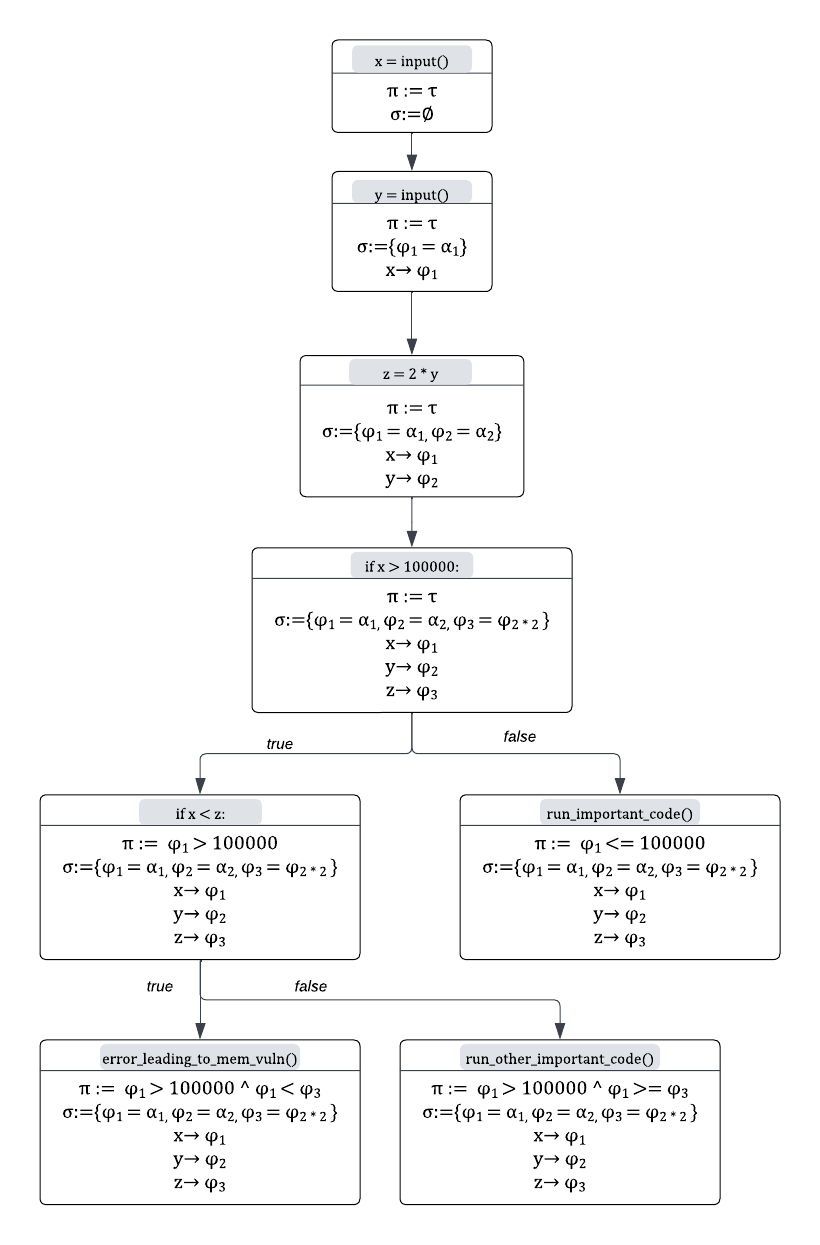
\includegraphics[scale=0.31]{figures/final_symbolic_example_graph.png}
        \caption{} % används för rendera b) som caption
        \label{fig:symbex_example_graph}
    \end{subfigure}

    \caption{Exempel för att visa symbolisk exekvering: pseudokod (a) och path
        constraint och symboliskt tillstånd för alla vägar i pseudokoden angett
        i (b). $  \mathcal{S} = \{\sigma := \{\phi_1 = \alpha_1, \phi_2 = \alpha_2, \phi_3 =
            2\phi_2\}, x \rightarrow \phi_1, y \rightarrow \phi_2, z \rightarrow
            \phi_3\}$}
\end{figure}

Exempelprogrammet i figur~\ref{fig:symbex_example_code} använder symbolisk
exekvering för att hitta vilken indata som leder programexekveringen till de
olika grenarna i programflödet. I många fall är det intressant att göra en
uttömmande sökning och hitta alla möjliga vägar i ett program, något som är
möjligt i detta program men inte i alla. Ett motexempel är komplexa
program som på grund av vägexplosionsproblemet inte hittar alla möjliga vägar.
Variablerna \emph{x} och \emph{y} sätts till symboliska värden som sedan används
för att beräkna vägvillkoret och de symboliska uttryck som variablerna utvecklas
till för en vald gren. Därefter används dessa uttryck och path constraints
tillsammans för att bilda en ekvation som sedan kan lösas med hjälp av en SMT-lösare.
Figur~\ref{fig:symbex_example_graph} visar
hur det symboliska tillståndet förändras för alla möjliga grenar i programmet.

I~\ref{fig:symbex_example_graph} används $\pi$ för att ange vägvillkoret vilket
är initialt satt till $\top$ eftersom villkoret är sant från början och $\sigma$
används för att visa mappningen för symboliska värden. $\pi$ och $\sigma$ % något man kan använda ist för mappning kanske
populeras längs med exekveringen, och \emph{x} och \emph{y} mappas till
symboliska värden. Beroende på vilken väg som väljs i exekveringen, uppdateras
vägvillkoret. I andra noden sett uppifrån finns det två skillnader i jämförelse
med den första noden: \emph{x} tilldelas $\phi_1$ som är en symbolisk mappning
till $\alpha_1$. Efter den fjärde noden sett uppifrån görs ett val och
vägvillkoret förändras beroende på vilken väg som tas -- vägvillkoret uppdateras
till $\phi_1 > 100000$ om $x < z$ och annars uppdateras det till $\phi_1 <=
    100000$. På samma sätt uppdateras $\pi$ och $\phi$ längs andra exekveringsvägar
och vilket till slut leder till ett komplett programflödesdiagram som beror på
\emph{x, y, z}. I varje nod kan ett konkret värde som uppfyller vägvillkoren evalueras.

\section{Fuzzing}
Fuzzing är ett användbart automatiskt verktyg för att testa program efter ofta
svårupptäckta problem som minnesbuggar, krascher, etc. tack vare dess enkelhet i
att konfigurera verktyget mot godtyckliga program.  

Grundprincipen i fuzzing är att attackera en större mängd av möjlig indata genom
att generera oväntad, godtycklig eller felaktig data. Denna typ av genererad
indata resulterar ofta i syntaktiskt eller semantiskt felaktig indata som inte
kan hanteras av målprogrammet. Således finns det anledning för
utvecklingspotential, något som lett till bland annat mutationsbaserad fuzzing
(jmf. eng. mutation-based fuzzing) och genereringsbaserad fuzzing (jmf. eng.
generation-based fuzzing). Mutationsbaserad fuzzing muterar känd giltig indata,
t.ex. om strängen 'fuzz' är giltig indata kan detta muteras till 'fuzzZZZZZ'. Om
en användare exempelvis vill fuzztesta bildhanteringsbiblioteket libjpeg skulle
detta innebära att skicka giltiga jpeg-bilder till fuzzern för att användas som
seeds, värden som används i pseudoslumptalsgeneratorer för att generera
pseudoslumptal, och sedan modifiera dessa. Detta skiljer sig från
genereringsbaserad fuzzing som genererar indata givet en modell för domänen --
en fördel i jämförelse med mutationsbaserad fuzzing som kräver känd kvalitativ
indata~\cite{fuzzing}. 

\subsection{Symbolisk fuzzing} Symbolisk fuzzing, eller concolic testing, är en
white-box fuzzermetod som nyttjar symbolisk exekvering för att maximera code
coverage -- fuzzerns förmåga att traversera över samtliga kanter och noder i
programmets kontrollflödesgraf. Skiljt från grey-box-fuzzers som AFL, möjliggör
symbolisk exekvering att fuzzern alltid väljer en branch som inte tidigare
tagits och således ökar code coverage~\cite{challenges_fuzzing}. Som beskrivet i
avsnittet \nameref{symbolisk_exekvering} sker detta genom att emulera programmet med hjälp av en virtuell
maskin och ersätta indata med symbolisk motsvarighet, som enklast beskrivs som
en liknelse till matematiska formler i form av ett algebraiskt uttryck. Dessa
uttryck bildar sedan tillsammans ett path constraint som skickas till en
SMT-lösare som resulterar i en input som leder till en given branch. 

\subsection{Problem med fuzzing} Ett problem är insikt om den underliggande
kodstrukturen. En viktig egenskap hos fuzzers som används för att beskriva dess
effektivitet är code coverage. Black-box-fuzzing är ett exempel på en fuzzer som
saknar vetskap om den underliggande kodstrukturen och genererar endast
slumpmässig indata, något som leder till ytlig testning av målprogrammet. I
kontrast till black-box-fuzzing finns det andra fuzzers, till exempel grey-box-fuzzern 
AFL~\cite{aflplusplus} som tillämpar binärinstrumentering, en teknik för
att observera eller manipulera en binär vilket görs genom att modifiera
källkoden i binären. Genom binärinstrumentering fås information om underliggande
basic blocks som delger övergången till nästa basic block. Detta används sedan
av AFL för att ge feedback till fuzzern som minns code coverage för en viss
indata och repeterar denna process för att maximera code coverage med ny indata
och därmed öka testytan~\cite{challenges_fuzzing}.

Fuzzers kräver ofta protokoll- eller domänkännedom för att kunna generera
indata. Detta blir problem för komplexa kodbaser eller bibliotek som saknar
trivial eller uppenbar indata och leder därmed till lägre code coverage. 

White-box fuzzers är inte en allmän lösning till problemen med fuzzing, utan
stretar med problem som exempelvis prestanda, path explosion, och falsk positiva
resultat. Det finns en stark korrelation mellan code coverage och bug
coverage~\cite{directed_greybox_fuzzing} men eftersom white-box fuzzing är ett
prestandakrävande verktyg kan detta leda till falsk positiva resultat genom att
resultatet från symboliska exekveringen guidar fuzzern längs med en branch som
inte nödvändigtvis leder till en bug, eller som är omöjlig. Trots existensen av
en stark korrelation mellan code coverage och bug coverage, innebär detta inte
att buggar kan uteslutas vid testning med hög code coverage. Det har visat sig
att enbart 3\% av Mozilla Firefox källkod innehåller
sårbarheter~\cite{fault_prediction_vuln_pred}, och därför är det oproduktivt att
blint följa code coverage.

\section{Statisk och dynamisk binäranalys}
En annan typ av kategorisering av olika analysmetoder som fokuserar på hur
analysen genomförs delar metoderna i två grupper: statisk och dynamisk
analys~\cite{dynamic_bin_analysis}.

Statisk analys syftar på analys som går att göra utan att exekvera programmet
som analyseras. Exempel på statisk binäranalys är metod 1--2, alltså att
disassembla binären och/eller visualisera kod~\cite{dynamic_bin_analysis}.

Dynamisk analys går ut på att analysera ett program under
exekvering~\cite{dynamic_bin_analysis}. Exempel på dynamisk binäranalys är
metod 3--6. I alla fall krävs någon typ av injektion av kod eller data i
programmet i syfte att kunna extrahera viktig information under programmets
körning~\cite{dynamic_bin_analysis}. Många avancerade dynamiska metoder som
t.ex.\ concolic testing kräver symbolisk exekvering som går ut på att tilldela
symboliska värden till variabler och se hur dessa påverkar programhopp och
förgreningar och vad för möjliga värden som denna symbol kan inneha under
exekvering. I fallet med concolic testing används denna information för att,
med hjälp av en SMT-solver ta fram konkreta värden som leder till att
programmet kör till en program-distination som består av ett krasch.

\section{Arkitektur för binäranalysverktyg}

Kärnan i ett korrekt dynamisk binäranalysverktyg är en
\emph{exekveringsmotor}, en komponent som på ett korrekt vis kan köra
programmet. Att köra ett program innebär att ladda binären och dess bibliotek,
hoppa till startadressen och sedan köra enskilda instruktioner. Om
binäranalysverktyget ska kunna använda metoder som använder symbolisk exekvering
behöver denna exekvering av enskilda instruktioner också stödja symboliska
variabler. För att verktyget ska uppnå hög prestanda är det eftersträvansvärt
att de instruktioner som inte använder symboliska variabler utan endast agerar
på konkreta värden exekverar direkt på processorn som kör binäranalysverktyget.

Program i verkligheten kommunicerar på många sätt med sin omgivning. För
inbyggda system är denna omgivning fysisk och för program som kör ovanpå
operativsystem är denna omgivning en virtuell värld bestående av filer och IPC (inter
process communication). För att en \textit{exekveringsmotor} ska vara så
brett tillämpbar som möjligt behöver den också stödja flera sorters
omgivningskommunikation.

Sammantaget är kraven på en exekveringsmotor med stöd för symbolisk analys att den
\begin{enumerate}
    \item kan ladda en binär i en konkret miljö;
    \item kan introducera symboliska variabler i denna miljö genom till exempel kommunikation med omgivningen;
    \item kan exekvera konkreta delar av programmet med god prestanda genom att köra dessa delar
          avprogrammet som maskinkod; och
    \item kan exekvera symboliska delar av programmet på ett sätt som är tillräckligt kraftfullt för de
          symboliska analyser som exekveringsmotorn ska användas till.
\end{enumerate}

Dessutom behöver exekveringsmotorn kunna kontrolleras och dess
slutsatser kunna användas av och presenteras i resten av programmet.
Figur~\ref{schematic} visar förhållandet mellan användaren, analysverktyget och
dess exekveringsmotor.

\begin{figure}[H]
    \centering
    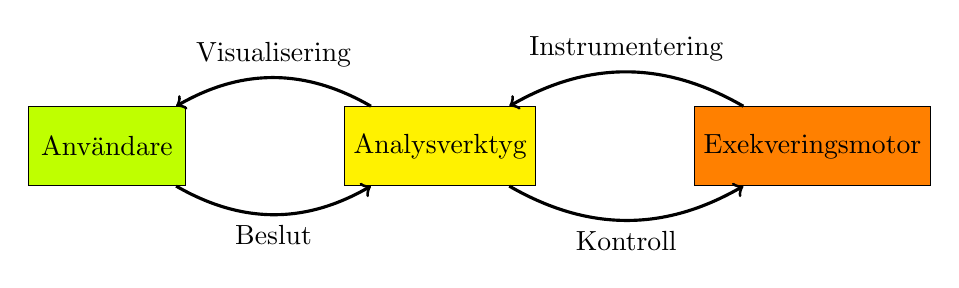
\begin{tikzpicture}

        \node [draw, fill=lime, minimum
            width=2cm, minimum height=1cm, ]  (user) {Användare};

        \node [draw, fill=yellow, minimum width=2cm, minimum height=1cm,
            right=2cm of user ] (tool) {Analysverktyg};

        \node [draw, fill=orange, minimum width=2cm, minimum height=1cm,
            right=2cm of tool ] (engine) {Exekveringsmotor};

        \draw[->, line width=.4mm] (user.-30) to[out=-30, in=-150]
        node[midway,below]{Beslut} (tool.-150);

        \draw[->, line width=.4mm] (tool.150) to[out=150, in=30]
        node[midway,above]{Visualisering} (user.30);

        \draw[->, line width=.4mm] (tool.-30) to[out=-30, in=-150]
        node[midway,below]{Kontroll} (engine.-150);

        \draw[->, line width=.4mm] (engine.150) to[out=150, in=30]
        node[midway,above]{Instrumentering} (tool.30);

    \end{tikzpicture}
    \caption{ Schematisk bild av ett binäranalysverktyg byggt kring en exekveringsmotor}\label{schematic}
\end{figure}

\subsection{Analyser}

Det finns många möjliga analyser som kan användas av ett binäranalysverktyg, där
\textit{analyser} avser en visualisering av en aspekt av det analyserade
programmets beteende eventuellt inklusive ett sätt för användaren att påverka
det analyserade programmets körning.

En konkret exekvering kan spåras och dess instruktionssekvens kan visas för
användaren med loopar identifierade. Flera exekveringar kan visualiseras på
samma sätt och deras instruktionssekvenser användas för att återskapa
kontrollflödesstrukturer som for- och while-loopar och if-satser.

Möjligheter för \textit{state merging} kan identifieras helautomatiskt eller av
användaren, alltså platser där flera exekveringar kan ersättas av en enda mer
generell exekvering som innehåller ursprungsexekveringarnas skillnader som
symboliska uttryck.

En uppsättning liknande exekveringar kan visas upp för användaren tillsammans
med information om när och hur de divergerar, för att till exempel avgöra när
olika delar av indatan används.

För analys av programmet är det också hjälpsamt för användaren att kunna stega
genom exekveringen steg för steg och ändra på värden för att ta de vägar de vill
analysera. Detta borde också kunna göras baklänges, det vill säga att användaren
väljer en slutdestination och låter programmet själv lista ut vilka värden som
behövdes läsas för att exekveringen skulle ta sig till den punkten.

En mer automatisk men ändå viktig funktionalitet är konstruktion av kod-täckande
indata. När testfall som besöker en uppsättning instruktioner är konstruerad kan
kraven på indatan över denna uppsättning programhopp analyseras och programmet
kan lista ut vilka aspekter av indatan som kan ändras utan att påverka
kodtäckningsgraden, och kommunicera detta till användaren.

Det finns många möjliga analyser. Användbarheten i ett verktyg mäts inte i
kvantiteten analyser utan i förmågan för de utvalda implementerade analyserna
att täcka användarens behov av förståelse av programmet.


\chapter{Existerande verktyg}
I avsnitt~\ref{sec:mal} beskriver vi projektets mål som att utveckla ett
binäranalysverktyg för att interaktivt visualisera symbolisk fuzztestning.
Visualiseringen presenteras i ett grafiskt gränssnitt där användaren kan
integrera med den virtulla maskinen som exekverar binären som analyseras.

Ett av projektets mål var att med visuella representationer av exekveringsstigar
göra det enklare för binäranalytikern att förstå binären. Med möjligheten att
ändra visualiseringen av en binärs kontrollflöde mellan fem olika grafer, och
därmed fem olika perspektiv. Idag uppnår AMBA det här målet under väldigt
begränsade förhållanden. Under arbetets gång observerade di att skapa ett
generellt visualiseringsverktyg av symbolisk fuzzingtestning är för omfattande
för att hinnas med under ett kandidatarbete. Med vidareutveckling, som
diskuteras mer i detalj i avsnitt~\ref{sec:vidareutveckling}, tror vi att AMBA
kommer vara praktiskt användbar under mer generella förhållanden.

Som diskuterat i avsnitt~\ref{sec:arbetsprocess} var ett av våra mål att
paketera AMBA tillsammans med dess komplexa beroenden. Att bygga AMBAs beroenden
visades vara mycket svårt då \stoe{}s bygginstruktioner är utdaterade och
fungerar inte längre. Till exempel hade \stoe{} projektets kopia av QEMU
flyttats, men länken hade inte uppdaterats i git vilket ledde till att kopian
behövde lokaliseras manuellt. Som nämnts i avsnitt \ref{sec:arbetsprocess} lades
även en ansenlig mängd tid på att försöka bygga guest images som skulle köras
inuti QEMU, men då vi inte lyckade producera samtliga artefakter beslutade vi
att använda de färdigbyggda guest images distribuerade av \stoe{} från Google
Drive. Då mycket tid behövde dedikeras till att korrigera byggsystemet innebar
det att mindre tid kunde allokeras till utveclandet av slutprodukten.

Vi försökte även minimera mängden \smallcaps{C++} kod som behövde skrivas genom
att använda Autocxx för att generera kopplingar mellan \smallcaps{C++} och Rust.
Tanken var att med hjälp av Autocxx skulle det endast ett fåtal rader
\smallcaps{C++}, och att merparten av källkoden skulle skrivas i Rust. Tyvärr
stötte vi på en bug i \smallcaps{Autocxx}, då den bland annat genererade
syntaktiskt inkorrekt kod. Då vi upptäckte att \smallcaps{Autocxx} saknade
viktiga funktioner beslutade vi oss efter några veckor att överge tanken att
generera kopplingar, för att skriva en större mängd \smallcaps{C++} kod.

Våra förhoppningar är att AMBA antingen kommer att vidareutvecklas, eller ligga
till grund för ett nytt verktyg, med funktionerna som diskuterades i avsnitt
\ref{sec:vidareutveckling}. För närvarande anser vi inte att AMBA är praktiskt
användbart, men att det finns en stor potential vid vidareutvecklingen av AMBA.

\section{Statisk disassemblering}
En vanlig statisk binäranalys är statisk disassemblering (ofta bara kallat
disassembering)\cite{andriesse2018}. Disassembering innebär att man försöker
återskapa assemblerinstruktioner frän maskinkoden i binären, utan att exekvera
maskinkoden\cite{andriesse2018}. En av svårigheterna med att översätta maskinkod
till assembler är att särskilda instruktioner från data\cite{andriesse2018}.
Till exempel kan man inte veta om maskinkoden \verb|0x8E| är värdet 0x8E (jrf.
142 i decimal) eller x86 intstruktionen \verb|mov|\cite{andriesse2018}. Det
finnr i huvudsak två metoder för att översätta maskininstruktioner
till assembler, \emph{linjär disassemblering}; och \emph{rekursiv
disassemblering}\cite{andriesse2018}.

Ghidra är ett \emph{reverse engingeering} ramverk utvecklat av NSA
(National Security Agency) och kan disassembla en binär till pseudo-C.
Ghidra har också en debugger och funktionsgraf. Debuggern ska underlätta binär
debugging genom att integrera med andra funktioner i Ghidra. Funktionsgrafen
låter användaren se hur programmet är uppbyggt visuellt och hur olika
funktioner interagerar med varandra. Funktionaliteter kan utökas eller andra
funktioner utvecklas genom plugins till Ghidra\cite{ghidra_use_cases}. Ghidra
tillåter även automatisering genom att skriva skript. Ett exempel är ett skript
som hittar exempelvis sårbarhet i form av funktionsanrop till potentiellt
osäkra API-anrop genom statisk analys\cite{ghidra_script}.

\section{Dynamiska binäranalysramverk}
En metod för dynamisk binäranalys är symbolisk exekvering. Eftersom exekveringen är symbolisk är
det möjligt att utforska alla möjliga exekveringsvägar i programmet, även de som inte är möjliga
med konkreta indata. Både \stoe{} och SymQEMU är kraftfulla verktyg för att analysera binära program
med symbolisk exekvering.

SymQEMU är byggt som en förlängning av QEMU, och använder en kombination av
dynamisk binäröversättning och symbolisk exekvering för att analysera binära
program som körs inuti emulatorn. SymQEMU utför kompileringsbaserad symbolisk
exekvering, där den mellanliggande representationen först blir modifierad innan
den översätts till värdarkitekturen, och är därför arkitekturoberoende utan att
påverka prestandan~\cite{symqemu}. Dessutom använder SymQEMU Linux user-mode
emulering, vilket innebär att endast användarutrymmet (jfr.\ eng.\ \emph{user space})
emuleras. Användarutrymmet innefattar alla program som inte körs av
operativsystemets kärna, och genom emulering nås högre prestanda i kontrast med
emulering av hela system~\cite{symqemu}.

\stoe{} är byggt ovanpå QEMU och utökar virtuella maskiner med stöd för
symbolisk exekvering. \stoe{} erbjuder redskap för att fokusera utforskningen på
delkomponenter av systemet och gör det även möjligt för användare att sätta in
kod i målsystemet vid specifika punkter under exekvering. Det gör att användare
kan anpassa analysprocessen efter sina behov~\cite{s2e}. \stoe{} kan analysera
kod för de flesta processorarkitekturer men betalar för det med ökad komplexitet
och prestanda~\cite{symqemu}.

I kontrast till SymQEMUs Linux user-mode emulering, emulerar \stoe{} hela
målsystemet, vilket innebär att \stoe{} kan göra analys på ett större antal
system. Inbyggda system är ett typexempel där det krävs helsystemsemulering då
bland annat inbyggda system ofta har modifierade operativsystem.

Ett annat verktyg för att identifiera buggar och sårbarheter med hjälp av dynamisk symbolisk
exekvering är SAGE (\emph{Scalable Automated Guided Execution}).
SAGE var det första verktyget som utförde dynamisk symbolisk exekvering på x86-binärnivå och använder flera
avgörande optimeringar för att hantera stora exekveringsspår (jfr.\ eng.\ \emph{execution traces}).
För att skala upp till stora exekveringsspår använder SAGE flera tekniker för att förbättra hastigheten och
minnesanvändningen för villkorsgenerering, exempelvis så kartläggs ekvivalenta symboliska uttryck till samma
objekt och villkor som redan är tillagda hoppas över~\cite{sage}.

Binäranalysverktyget angr stödjer både statiska analyser såsom dekompilering
till pseudo-C-kod och dynamiska analyser med hjälp av symbolisk exekvering.
Användarens analyser utförs genom Python-skript som interagerar med angrs API
för att kontrollera en symbolisk emulator skriven i Python för angr. Skript som
använder angr kan användas för \emph{reverse engineering}, sårbarhetssökning och
kan även vara del av exploateringsverktyg~\cite{angr_docs}. Tävlingen Cyber
Grand Challenge organiserades 2016 av DARPA.\@ I tävlingen skulle lag skriva
helautomatiska system som hittar, korrigerar och angriper sårbarheter i
CTF-liknande uppgifter.  Det vinnande systemet, Mayhem, använde angr som
symbolisk exekveringsmotor.

För att accelerera den symboliska exekveringen kan angr användas i kombination
med Unicorn CPU-emulatorn, ett lättviktigt ramverk för emulering som stödjer
många arkitekturer och baseras på QEMU~\cite{UnicornEngine}. Detta är möjligt
med hjälp av komponenten \emph{angr.engines.unicorn}. Genom att använda
komponenten kan man exekvera med konkreta indata när det är möjligt och
fördelaktigt men understött av symbolisk exekvering då flera exekveringsvägar
behöver utforskas eller då programmets beteende inte är
deterministiskt~\cite{angrUnicornEngine}. I angr kan det emulerade programmet
manipulera filer och nätverksströmmar som representeras som Python-objekt. Dessa
objekt läses från och skrivs till när det emulerade programmet utför
systemanrop.


\chapter{AMBA}
I avsnitt~\ref{sec:mal} beskriver vi projektets mål som att utveckla ett
binäranalysverktyg för att interaktivt visualisera symbolisk fuzztestning.
Visualiseringen presenteras i ett grafiskt gränssnitt där användaren kan
integrera med den virtulla maskinen som exekverar binären som analyseras.

Ett av projektets mål var att med visuella representationer av exekveringsstigar
göra det enklare för binäranalytikern att förstå binären. Med möjligheten att
ändra visualiseringen av en binärs kontrollflöde mellan fem olika grafer, och
därmed fem olika perspektiv. Idag uppnår AMBA det här målet under väldigt
begränsade förhållanden. Under arbetets gång observerade di att skapa ett
generellt visualiseringsverktyg av symbolisk fuzzingtestning är för omfattande
för att hinnas med under ett kandidatarbete. Med vidareutveckling, som
diskuteras mer i detalj i avsnitt~\ref{sec:vidareutveckling}, tror vi att AMBA
kommer vara praktiskt användbar under mer generella förhållanden.

Som diskuterat i avsnitt~\ref{sec:arbetsprocess} var ett av våra mål att
paketera AMBA tillsammans med dess komplexa beroenden. Att bygga AMBAs beroenden
visades vara mycket svårt då \stoe{}s bygginstruktioner är utdaterade och
fungerar inte längre. Till exempel hade \stoe{} projektets kopia av QEMU
flyttats, men länken hade inte uppdaterats i git vilket ledde till att kopian
behövde lokaliseras manuellt. Som nämnts i avsnitt \ref{sec:arbetsprocess} lades
även en ansenlig mängd tid på att försöka bygga guest images som skulle köras
inuti QEMU, men då vi inte lyckade producera samtliga artefakter beslutade vi
att använda de färdigbyggda guest images distribuerade av \stoe{} från Google
Drive. Då mycket tid behövde dedikeras till att korrigera byggsystemet innebar
det att mindre tid kunde allokeras till utveclandet av slutprodukten.

Vi försökte även minimera mängden \smallcaps{C++} kod som behövde skrivas genom
att använda Autocxx för att generera kopplingar mellan \smallcaps{C++} och Rust.
Tanken var att med hjälp av Autocxx skulle det endast ett fåtal rader
\smallcaps{C++}, och att merparten av källkoden skulle skrivas i Rust. Tyvärr
stötte vi på en bug i \smallcaps{Autocxx}, då den bland annat genererade
syntaktiskt inkorrekt kod. Då vi upptäckte att \smallcaps{Autocxx} saknade
viktiga funktioner beslutade vi oss efter några veckor att överge tanken att
generera kopplingar, för att skriva en större mängd \smallcaps{C++} kod.

Våra förhoppningar är att AMBA antingen kommer att vidareutvecklas, eller ligga
till grund för ett nytt verktyg, med funktionerna som diskuterades i avsnitt
\ref{sec:vidareutveckling}. För närvarande anser vi inte att AMBA är praktiskt
användbart, men att det finns en stor potential vid vidareutvecklingen av AMBA.


\chapter{Implementation}
I avsnitt~\ref{sec:mal} beskriver vi projektets mål som att utveckla ett
binäranalysverktyg för att interaktivt visualisera symbolisk fuzztestning.
Visualiseringen presenteras i ett grafiskt gränssnitt där användaren kan
integrera med den virtulla maskinen som exekverar binären som analyseras.

Ett av projektets mål var att med visuella representationer av exekveringsstigar
göra det enklare för binäranalytikern att förstå binären. Med möjligheten att
ändra visualiseringen av en binärs kontrollflöde mellan fem olika grafer, och
därmed fem olika perspektiv. Idag uppnår AMBA det här målet under väldigt
begränsade förhållanden. Under arbetets gång observerade di att skapa ett
generellt visualiseringsverktyg av symbolisk fuzzingtestning är för omfattande
för att hinnas med under ett kandidatarbete. Med vidareutveckling, som
diskuteras mer i detalj i avsnitt~\ref{sec:vidareutveckling}, tror vi att AMBA
kommer vara praktiskt användbar under mer generella förhållanden.

Som diskuterat i avsnitt~\ref{sec:arbetsprocess} var ett av våra mål att
paketera AMBA tillsammans med dess komplexa beroenden. Att bygga AMBAs beroenden
visades vara mycket svårt då \stoe{}s bygginstruktioner är utdaterade och
fungerar inte längre. Till exempel hade \stoe{} projektets kopia av QEMU
flyttats, men länken hade inte uppdaterats i git vilket ledde till att kopian
behövde lokaliseras manuellt. Som nämnts i avsnitt \ref{sec:arbetsprocess} lades
även en ansenlig mängd tid på att försöka bygga guest images som skulle köras
inuti QEMU, men då vi inte lyckade producera samtliga artefakter beslutade vi
att använda de färdigbyggda guest images distribuerade av \stoe{} från Google
Drive. Då mycket tid behövde dedikeras till att korrigera byggsystemet innebar
det att mindre tid kunde allokeras till utveclandet av slutprodukten.

Vi försökte även minimera mängden \smallcaps{C++} kod som behövde skrivas genom
att använda Autocxx för att generera kopplingar mellan \smallcaps{C++} och Rust.
Tanken var att med hjälp av Autocxx skulle det endast ett fåtal rader
\smallcaps{C++}, och att merparten av källkoden skulle skrivas i Rust. Tyvärr
stötte vi på en bug i \smallcaps{Autocxx}, då den bland annat genererade
syntaktiskt inkorrekt kod. Då vi upptäckte att \smallcaps{Autocxx} saknade
viktiga funktioner beslutade vi oss efter några veckor att överge tanken att
generera kopplingar, för att skriva en större mängd \smallcaps{C++} kod.

Våra förhoppningar är att AMBA antingen kommer att vidareutvecklas, eller ligga
till grund för ett nytt verktyg, med funktionerna som diskuterades i avsnitt
\ref{sec:vidareutveckling}. För närvarande anser vi inte att AMBA är praktiskt
användbart, men att det finns en stor potential vid vidareutvecklingen av AMBA.


\chapter{Evaluering}
I avsnitt~\ref{sec:mal} beskriver vi projektets mål som att utveckla ett
binäranalysverktyg för att interaktivt visualisera symbolisk fuzztestning.
Visualiseringen presenteras i ett grafiskt gränssnitt där användaren kan
integrera med den virtulla maskinen som exekverar binären som analyseras.

Ett av projektets mål var att med visuella representationer av exekveringsstigar
göra det enklare för binäranalytikern att förstå binären. Med möjligheten att
ändra visualiseringen av en binärs kontrollflöde mellan fem olika grafer, och
därmed fem olika perspektiv. Idag uppnår AMBA det här målet under väldigt
begränsade förhållanden. Under arbetets gång observerade di att skapa ett
generellt visualiseringsverktyg av symbolisk fuzzingtestning är för omfattande
för att hinnas med under ett kandidatarbete. Med vidareutveckling, som
diskuteras mer i detalj i avsnitt~\ref{sec:vidareutveckling}, tror vi att AMBA
kommer vara praktiskt användbar under mer generella förhållanden.

Som diskuterat i avsnitt~\ref{sec:arbetsprocess} var ett av våra mål att
paketera AMBA tillsammans med dess komplexa beroenden. Att bygga AMBAs beroenden
visades vara mycket svårt då \stoe{}s bygginstruktioner är utdaterade och
fungerar inte längre. Till exempel hade \stoe{} projektets kopia av QEMU
flyttats, men länken hade inte uppdaterats i git vilket ledde till att kopian
behövde lokaliseras manuellt. Som nämnts i avsnitt \ref{sec:arbetsprocess} lades
även en ansenlig mängd tid på att försöka bygga guest images som skulle köras
inuti QEMU, men då vi inte lyckade producera samtliga artefakter beslutade vi
att använda de färdigbyggda guest images distribuerade av \stoe{} från Google
Drive. Då mycket tid behövde dedikeras till att korrigera byggsystemet innebar
det att mindre tid kunde allokeras till utveclandet av slutprodukten.

Vi försökte även minimera mängden \smallcaps{C++} kod som behövde skrivas genom
att använda Autocxx för att generera kopplingar mellan \smallcaps{C++} och Rust.
Tanken var att med hjälp av Autocxx skulle det endast ett fåtal rader
\smallcaps{C++}, och att merparten av källkoden skulle skrivas i Rust. Tyvärr
stötte vi på en bug i \smallcaps{Autocxx}, då den bland annat genererade
syntaktiskt inkorrekt kod. Då vi upptäckte att \smallcaps{Autocxx} saknade
viktiga funktioner beslutade vi oss efter några veckor att överge tanken att
generera kopplingar, för att skriva en större mängd \smallcaps{C++} kod.

Våra förhoppningar är att AMBA antingen kommer att vidareutvecklas, eller ligga
till grund för ett nytt verktyg, med funktionerna som diskuterades i avsnitt
\ref{sec:vidareutveckling}. För närvarande anser vi inte att AMBA är praktiskt
användbart, men att det finns en stor potential vid vidareutvecklingen av AMBA.

\section{Metod}

I avsikt att utveckla ett binäranalysverktyg, bestämdes det att ta fram demon
(demonstrationer) som ska leda det kontinuerliga utvecklingsarbetet.

Ett demo ska bestå av en analys med hjälp av verktyget som ökar förståelse för
ett exempelprogram. Med förståelse menas en abstrakt programförståelse
beskrivet i bakgrundsavsnittet. Exempelprogrammet ska framställas med en
egenskap som man skulle vilja kunna detektera med ett analysverktyg. Mer
konkret ska ett sådant exempelprogram inneha t.ex. minnessårbarhet, ett oväntad
krasch eller något annat sårbarhet som inte önskas i ett program.

Exempelprogrammen ska skrivas i C för enkelhetens skull eftersom C-programs
utseende i binärformat relativt väl motsvarar deras källkod. 

Sedan ska exempelprogrammet kompileras till en binär som analyseras med
analysverktyget med avsikt att detektera den kända egenskapen hos
exempelprogrammet. Om detta inte är möjligt med den nuvarande version av
analysverktyget ska analysverktyget utökas för att möjliggöra demot.

Detta tillvägagångssätt är önskvärt eftersom det tillåter att sätta uppnåbara
delmål som styr funktionalitet i analysverktyget som ska implementeras härnäst.
Dessutom kan flera demon utvecklas samtidigt vilket tillåter parallellism inom
utvecklingen och framsteg på flera fronter.

Tillvägagångssättet är jämförbart med den agila arbetsmetoden där utveckling sker 
evolutionärt. Detta är önskvärt då verktygets potentiella 
användningsbarhet inte är självklar på detaljnivå.

I ett senare och/eller parallellt steg ska ett grafiskt användargränssnitt
utvecklas som tillåter användaren att navigera programmet som analyseras och
göra egna beslut gällande förgreningar etc. där användaren själv bestämmer
interaktivt nästa beslut som görs. Även detta arbete styrs av demon som
framställs och funktionaliteter som önskas.

\subsection{Evaluering och jämförelse med andra verktyg}

För att det ska gå att testa verktygets förmåga och jämföra med andra
analysverktyg ska de demon som tas fram bestå av CGC-binärer som analyseras. I
det fall CGC-binären är för komplicerat ska den förenklas samtidigt som den
originala sårbarheten återfinns, eller delas in i flera demon, tills dess att
den kompletta CGC-binären kan analyseras och sårbarheten detekteras.

Samma CGC-binärer som kan analyseras med det framställda analysverktyget ska
analyseras med binäranalysverktygen \emph{Angr} och \emph{Ghidra} och
analysresultatet jämföras för att göra en kvalitativ evaluering av eventuella
för- och nackdelar med det framtagna analysverktyget jämfört med de ovan nämnda
existerande verktygen. Jämförelsen kommer att ta hänsyn till hur snabbt det
gick att genomföra analysen, hur mycket ansträngning det krävde från
användaren, om det överhuvudtaget gick att hitta sårbarheten i CGC-binären, och
eventuellt andra för och nackdelar.

Val av CGC-binärer att analysera kommer att vara slumpmässigt med undantag för
fall då det anses ta för långt tid att utveckla vårt verktyg för att tillåta
analys av programmet med hänsyn till tidsbegränsningen för detta projekt.

\section{Begränsningar}
\input{evaluering/begransningar.tex}

\chapter{Slutsats}
I avsnitt~\ref{sec:mal} beskriver vi projektets mål som att utveckla ett
binäranalysverktyg för att interaktivt visualisera symbolisk fuzztestning.
Visualiseringen presenteras i ett grafiskt gränssnitt där användaren kan
integrera med den virtulla maskinen som exekverar binären som analyseras.

Ett av projektets mål var att med visuella representationer av exekveringsstigar
göra det enklare för binäranalytikern att förstå binären. Med möjligheten att
ändra visualiseringen av en binärs kontrollflöde mellan fem olika grafer, och
därmed fem olika perspektiv. Idag uppnår AMBA det här målet under väldigt
begränsade förhållanden. Under arbetets gång observerade di att skapa ett
generellt visualiseringsverktyg av symbolisk fuzzingtestning är för omfattande
för att hinnas med under ett kandidatarbete. Med vidareutveckling, som
diskuteras mer i detalj i avsnitt~\ref{sec:vidareutveckling}, tror vi att AMBA
kommer vara praktiskt användbar under mer generella förhållanden.

Som diskuterat i avsnitt~\ref{sec:arbetsprocess} var ett av våra mål att
paketera AMBA tillsammans med dess komplexa beroenden. Att bygga AMBAs beroenden
visades vara mycket svårt då \stoe{}s bygginstruktioner är utdaterade och
fungerar inte längre. Till exempel hade \stoe{} projektets kopia av QEMU
flyttats, men länken hade inte uppdaterats i git vilket ledde till att kopian
behövde lokaliseras manuellt. Som nämnts i avsnitt \ref{sec:arbetsprocess} lades
även en ansenlig mängd tid på att försöka bygga guest images som skulle köras
inuti QEMU, men då vi inte lyckade producera samtliga artefakter beslutade vi
att använda de färdigbyggda guest images distribuerade av \stoe{} från Google
Drive. Då mycket tid behövde dedikeras till att korrigera byggsystemet innebar
det att mindre tid kunde allokeras till utveclandet av slutprodukten.

Vi försökte även minimera mängden \smallcaps{C++} kod som behövde skrivas genom
att använda Autocxx för att generera kopplingar mellan \smallcaps{C++} och Rust.
Tanken var att med hjälp av Autocxx skulle det endast ett fåtal rader
\smallcaps{C++}, och att merparten av källkoden skulle skrivas i Rust. Tyvärr
stötte vi på en bug i \smallcaps{Autocxx}, då den bland annat genererade
syntaktiskt inkorrekt kod. Då vi upptäckte att \smallcaps{Autocxx} saknade
viktiga funktioner beslutade vi oss efter några veckor att överge tanken att
generera kopplingar, för att skriva en större mängd \smallcaps{C++} kod.

Våra förhoppningar är att AMBA antingen kommer att vidareutvecklas, eller ligga
till grund för ett nytt verktyg, med funktionerna som diskuterades i avsnitt
\ref{sec:vidareutveckling}. För närvarande anser vi inte att AMBA är praktiskt
användbart, men att det finns en stor potential vid vidareutvecklingen av AMBA.


\printbibliography

\end{document}
